%crossrefs
%1
%bib done
%examples done
%tables done
%crossrefs 

\section{Introduction}\label{sec:1:1}
The languages of the Alor-Pantar (AP) family constitute a group of twenty Papuan languages spoken on the islands of Alor and Pantar, located just north of Timor, at the end of the Lesser Sunda island chain, roughly the islands east of Bali and west of New Guinea, see Figure \ref{fig:1:Map1}. This outlier ``Papuan'' group is located some 1000 kilometers west of the New Guinea mainland. The term \textit{Papuan} is used here as a cover term for the hundreds of languages spoken in New Guinea and its vicinity that are not Austronesian \citep[15]{Ross2005}, and it is considered synonymous with non-Austronesian. The label \textit{Papuan} says nothing about the genealogical ties between the languages. 

The Alor-Pantar languages form a family that is clearly distinct from the Austronesian languages\il{Austronesian language(s)} spoken on the islands surrounding Alor and Pantar, but much is still unknown about their history: Where did they originally come from? Are they related to other languages or language groups, and if so, to which ones? Typologically, the AP languages are also very different from their Austronesian neighbours, as their syntax is head-final rather than a head-initial. They show an interesting variety of alignment patterns, and the family has some cross-linguistically rare features.  

This volume studies the history and typology of the AP languages. Each chapter compares a set of AP languages by their lexicon, syntax or morphology, with the aim to uncover linguistic history and discover typological patterns that inform linguistic theory. 

As an introduction to the volume, this chapter places the AP languages in their current linguistic context ({\S{}} \ref{sec:1:2}), followed by an overview of the history of research in the area ({\S{}} \ref{sec:1:3}). Then I describe the state of the art of the (pre-)history of speaker groups on Alor and Pantar ({\S{}} \ref{sec:1:4}). A typological overview of the family is presented in {\S{}} \ref{sec:1:5}, followed by information on the lexicon in {\S{}} \ref{sec:1:6}. In {\S{}} \ref{sec:1:7}, I summarize the chapter and outline challenges for future research in the area. The chapter ends with a description of the empirical basis for the research that is reported in this volume ({\S{}} \ref{sec:1:8}). Throughout this introduction, cross-references to the chapters will be given, to enable the reader to focus on those chapters that s/he is most interested in. 


\begin{figure}
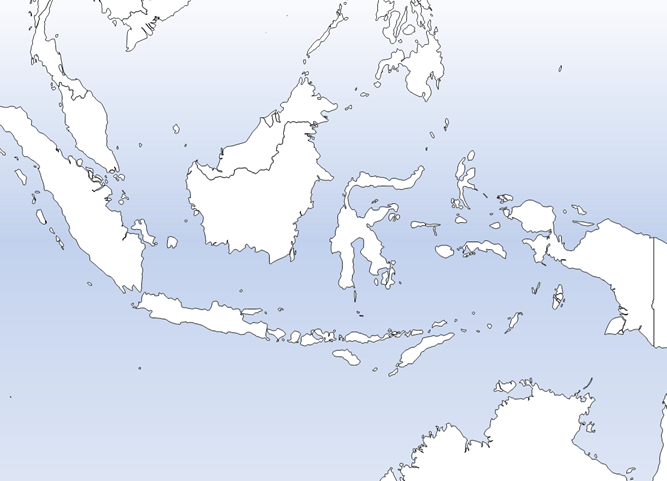
\includegraphics[width=\textwidth]{figures/klamer_ch1_fig1.png}
\caption{Alor and Pantar in Indonesia}
\label{fig:1:Map1}
\end{figure}  



\section{Current linguistic situation on Alor and Pantar}\label{sec:1:2}
There are approximately 20 indigenous Papuan languages spoken in the Alor-Pantar archipelago ({\S} 2.1) alongside one large indigenous Austronesian language\il{Austronesian language(s)} commonly referred to as Alorese\il{Alorese} ({\S} 2.2). Virtually all speakers of these indigenous languages also speak the local Malay variety\il{Malay} and/or the national language Indonesian\il{Indonesian} on a regular basis for trade, education and governmental business ({\S} \ref{sec:1:2.3}). 

\subsection{The Papuan languages of Alor and Pantar} \label{sec:1:2.1}
The Papuan languages of Alor and Pantar as they are currently known are listed alphabetically in Table \ref{tab:1:1}, and presented geographically on Figure \ref{fig:1:Map2}. Together they form the Alor-Pantar family. The Alor-Pantar family forms a higher-order family grouping with the five Papuan languages spoken on Timor and Kisar, listed in Table \ref{tab:1:2} and presented geographically on Figure \ref{fig:1:Map3}; together these languages constitute the Timor-Alor-Pantar family.

The language list in Table \ref{tab:1:1} is a preliminary one. In particular, it is likely that the central-eastern part of Alor, where Abui\il{Abui} and Kamang\il{Kamang} are spoken, is linguistically richer than suggested by Table \ref{tab:1:1} and Figure \ref{fig:1:Map2}. However, until a more principled survey of the area has been done, we stick with the labels Abui and Kamang, while acknowledging that there may be multiple languages within each of these regions.

Some of the language names of earlier works (e.g. \citealt{Stokhof1975}, \citealt{GrimesEtAl1997}, \citealt{LewisEtAl2013}) do not agree with what is presented here (see also {\S} \ref{sec:1:3}). One reason may be that a language variety may either be referred to by the name of the village where it is spoken, or by the name of the ancestor village of the major clan that speaks the language, or by the clan name. The list in Table \ref{tab:1:1} aims toward more `lumping' than `splitting'. The traditional criterion of mutual intelligibility is extremely difficult to apply, as speakers of the languages have been in contact for extended periods of time, and being multi-lingual is the norm in this region.

For those languages which have been the subject of recent investigation a reference is included in the table to a grammar or grammatical sketch that is published, or is about to be published. Further references to published work on the languages are presented in {\S} 3.



\begin{table}\centering
\begin{tabular}{p{2.6cm}p{.9cm}p{1.7cm}lp{3.3cm}}
\mytoprule
{Language}\footnotemark{} & {ISO\newline639-3} & {Alternate   Name(s)} & {Pop.}\footnotemark{} & {References \par (selected)}\\
\midrule 
Abui\ilt{Abui} (A\textsc{b}) & abz & Papuna & 17000 & \citet{Kratochvil2007} \\
Adang\ilt{Adang} (A\textsc{d}) & adn &  & 7000 &{}\citet{Haan2001,RobinsonEtAltaadang} \\
Blagar\ilt{Blagar} (B\textsc{l}) & beu & Pura & 10000 &{}{\citet{Steinhauerta}} \\
Deing\ilt{Deing} (D\textsc{e}) & -- & Diang, Tewa & {}-{}- & \\
Hamap\ilt{Hamap} (H\textsc{m}) & hmu &  & 1300* & \\
Kabola\ilt{Kabola} (K\textsc{b}) & klz &  & 3900* &\citet{Stokhof1987} \\
Kaera\ilt{Kaera} (K\textsc{e}) & -- &  & 5500 &\citet{Klamertakaera}\\
Kafoa\ilt{Kafoa} (K\textsc{f}) & kpu &  & 1000* &{}\citet{Bairdta} \\
Kamang\ilt{Kamang} (K\textsc{m}) & woi & Woisika & 6000 &{}\citet{Stokhof1977,Schapperta} \\
Kiramang\ilt{Kiraman} (K\textsc{r}) & kvd &  & 4240* & \\
Klon\ilt{Klon} (K\textsc{l}) & kyo & Kelon & 5000 &{}\citet{Baird2008} \\
Kui\ilt{Kui} (K\textsc{i}) & kvd &  & 4240* & \\
Kula\ilt{Kula} (K\textsc{u}) & tpg & Tanglapui & 5000* &{}\citet{WilliamsEtAlta,Donohue1996} \\
Nedebang\ilt{Nedebang} (N\textsc{d}) & nec & Klamu & 1380* & \\
Reta\ilt{Reta} (R\textsc{t}) & ret & Retta & 800 & \\
Sar\ilt{Sar} (S\textsc{r}) & {}-{}- & Teiwa? & {}-{}- & \\
Sawila\ilt{Sawila} (S\textsc{w}) & swt &  & 3000 &{}\citet{Kratochvilta} \\
Teiwa\ilt{Teiwa} (T\textsc{w}) & twe & Tewa & 4000 &{}\citet{Klamer2010grammar} \\
Wersing\ilt{Wersing} (W\textsc{e}) & kvw & Kolana & 3700* &{}\citet{SchapperEtAltawersing} \\
Western \newline Pantar (WP)\ilt{Western Pantar} & lev & Lamma, Tubbe, Mauta, Kalondama & 10300\footnotemark{} &{}{\citet{Holton2010person,Holtontanumeral}} \\
\mybottomrule
\end{tabular}
\caption{The languages of the Alor-Pantar family.}
\label{tab:1:1}
\end{table}

\addtocounter{footnote}{-3}
\stepcounter{footnote}\footnotetext{The abbreviations in brackets are used to refer to the languages in the historical comparative chapters by \citet{HoltonRobinsonTVhistory,HoltonRobinsonTVposition} and \citet{SchapperEtAlTVtimor}}. 
\stepcounter{footnote}\footnotetext{Population estimates from fieldworker and/or from the published source given; starred (*) estimates from \citet{LewisEtAl2013}; an empty cell indicates that no number has been reported.}
\stepcounter{footnote}\footnotetext{This figure is from census data \citep{BadanPusat2005}.} 

\begin{figure} 
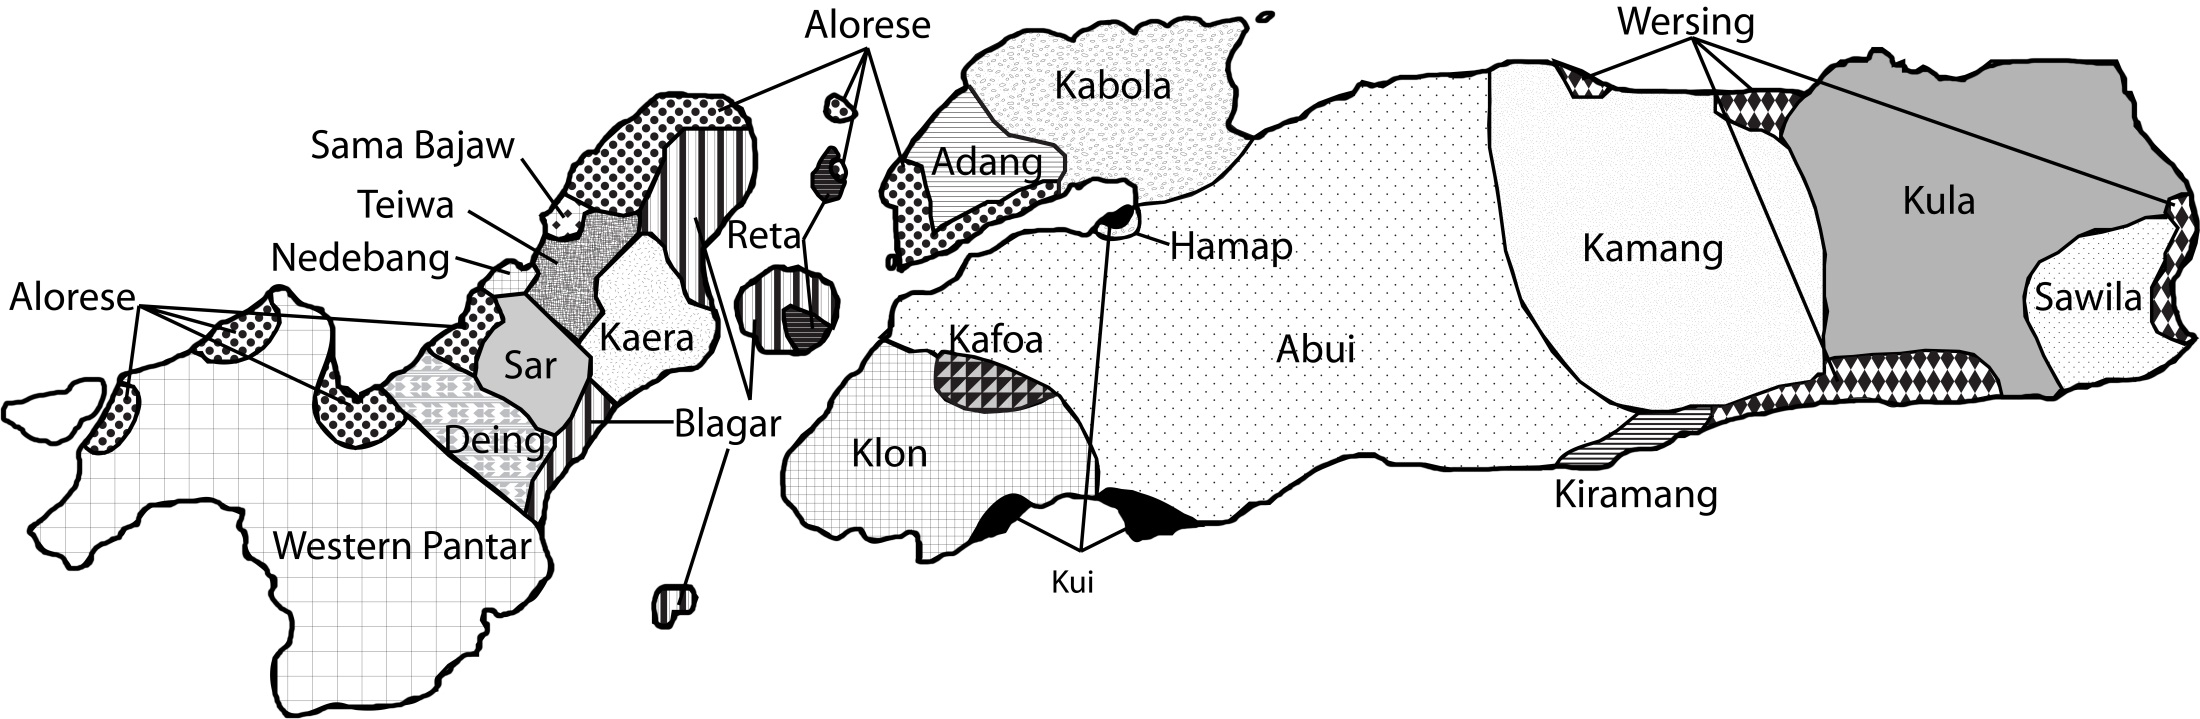
\includegraphics[width=\textwidth]{figures/klamer_ch1_fig2.png}
\caption{The languages of the Alor-Pantar family, and Austronesian\ilt{Austronesian language(s)} Alorese\ilt{Alorese}.}
\label{fig:1:Map2}
\end{figure} 



\begin{table}\centering
\begin{tabular}{p{2.6cm}p{.9cm}p{1.7cm}lp{3.3cm}}
\mytoprule
{Language} & {ISO} \newline {639-3} & {Alternate} \newline{Name(s)} & {Pop.}\footnotemark{} & {References (selected\-)}\\
\midrule 
Bunaq\ilt{Bunaq} & bfn & Buna('), Bunak(e) & 80.000* &\citet{Schapper2009} \\
Fataluku\ilt{Fataluku} & ddg &  & 30000* &\citet{VanEngelenhoven2009,VanEngelenhoven2010} \\
Makalero\ilt{Makalero} & mkz & Maklere & 6500* &\citet{Huber2011} \\
Makasai\ilt{Makasae} & mkz & Makasae & 70000* &\citet{Huber2008} \\
Oirata\ilt{Oirata} & oia &  & 1220* & \citet{DeJong1937} \\
\mybottomrule
\end{tabular}
\caption{The Papuan languages of Timor and Kisar.}
\label{tab:1:2}
\end{table}

\footnotetext{Population estimates from fieldworker and/or from the published source given; starred (*) estimates from \citet{LewisEtAl2013}.}



\begin{figure}
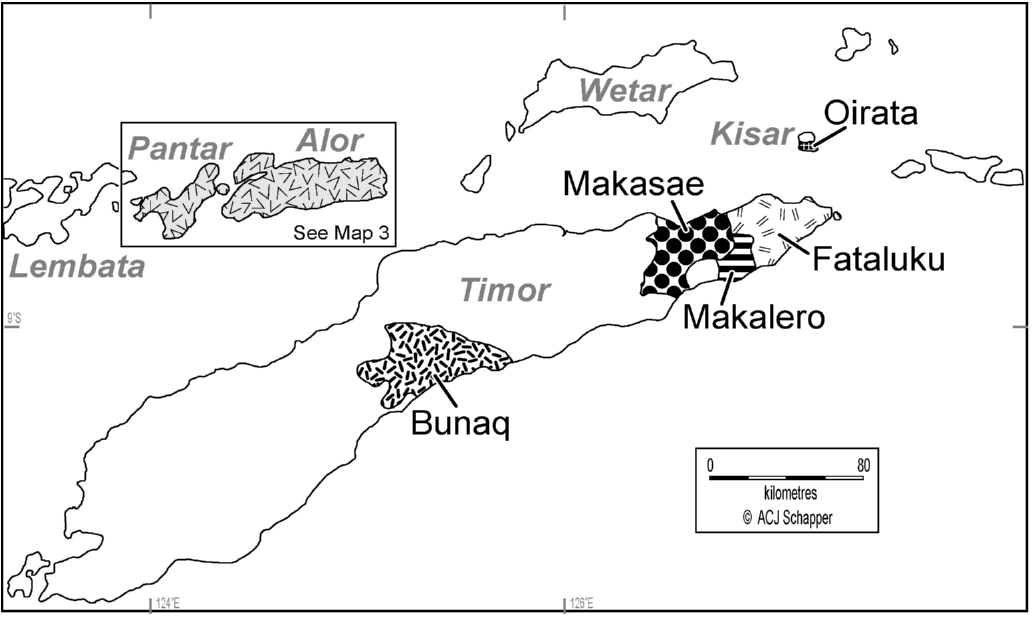
\includegraphics[width=\textwidth]{figures/klamer_ch1_fig3.png}

\caption{The Papuan languages of Timor-Alor-Pantar. (Areas where Austronesian languages\ilt{Austronesian language(s)} are spoken are left white.)}
\label{fig:1:Map3}
\end{figure} 






\subsection{Indigenous Austronesian languages\ilt{Austronesian language(s)} on Alor and Pantar} \label{sec:1:2.2}
The major indigenous Austronesian language\il{Austronesian language(s)} spoken on Alor and Pantar is Alorese\il{Alorese}, also referred to as \textit{Bahasa Alor}, `Alor', or `Coastal Alorese'. \citet{Klamer2011} is a sketch of the language. Alorese has 25,000 speakers, who live in pockets along the coasts of western Pantar and the Kabola peninsula of Alor island, as well as on the islets Ternate and Buaya (\citealt[8-9]{Stokhof1975},\citealt{GrimesEtAl1997,Lewis2009}). There are reports that Alorese was used as the language of wider communication in the Alor-Pantar region until at least the mid 1970s \citep[see][8]{Stokhof1975}, but as such it did not make inroads into the central mountainous areas of Pantar or Alor, and its lingua franca function may have been limited to Pantar and the Straits in between Pantar and Alor.

The vocabulary of Alorese\il{Alorese} is clearly (Malayo-Polynesian) Austronesian\il{Austronesian language(s)}. On the basis of a short word list, \citet[9]{Stokhof1975} and \citet[645]{Steinhauer1993} suggest that the language spoken on the Alor and Pantar coasts is a dialect of Lamaholot\il{Lamaholot}. Lamaholot is an Austronesian language spoken on the islands west of Pantar: Lembata, Solor, Adonara, and East Flores.\footnote{Note that both \citet[275]{Barnes2001} and \citet[82]{Blust2009}, \citet[87]{Blust2013} indicate that Lamaholot is spoken on the Alor and Pantar coasts; in actual fact this is Alorese \citep[cf.][]{Klamer2011}.} Recent research however indicates that Alorese and Lamaholot show significant differences in lexicon as well as grammar: Alorese and Lamaholot share only 50-60\% of their basic vocabulary, severely hindering mutual intelligibility; the languages have different sets of pronouns\is{pronoun} and different possessive constructions\is{possession}; and, most striklingly, Alorese\il{Alorese} lacks all the inflectional\is{inflection} and derivational morphology\is{derivation} that is present in Lamaholot\il{Lamaholot} \citep{Klamer2011,Klamer2012}. The evidence clearly suggests that Alorese should be considered a language in its own right. 

Oral history and ethnographic observations \citep{Anonymous1914,Lemoine1969,Rodemeier2006} report local traditions about non-indigenous, Austronesian groups arriving in {the northern coastal parts of Pantar around 1,300 AD whose} descendants colonized the coasts of north-western Pantar and west Alor. Some of the locations mentioned are home to speakers of Alorese.\footnote{Pandai, Baranusa and Alor are locations where Alorese is spoken today. \citet[38]{Hagerdal2012} cites evidence that Kui and Blagar were part of the league of princedoms with Pandai, Baranusa, and Alor.}    

Apart from Alorese, there are also languages spoken by more recent Austronesian immigrants. For instance, Bajau\il{Bajau} (or Bajo) is the language of the nomadic communities located throughout most of Indonesia which are also referred to as `sea gypsies' \citep[cf.][]{Verheijen1986}. There are reports that there has been a community of Bajau\il{Bajau} on Pantar since the early 1800s (Laura Robinson p.c.). One or more groups of Bajau came from Sulawesi, through Flores, and settled on the coast near Kabir, on Pantar island, in the 1950s. A second wave of Bajau speakers arrived from East Timor in 1999. Bajau communities are also found on Alor. 

\subsection{Indonesian and Alor Malay}\label{sec:1:2.3}
Indonesian\il{Indonesian} has been introduced relatively recently in the Alor-Pantar region, roughly correlating with the increasing number of Indonesian primary schools established in rural areas since the 1960s. Today, speakers of the Alor Pantar languages employ Indonesian and/or the local variety of Malay\il{Malay} as language of trade, education, and governmental business. 

The Alor Malay variety was already in use in the Alor-Pantar archipelago before standard Indonesian was introduced. Alor Malay is based on the Malay variety spoken in Kupang, the capital of the Indonesian province Nusa Tenggara Timor (NTT)\is{Nusa Tenggara Timor} which is located on Timor island \citep{JacobEtAl2003,BairdEtAlMs}, though there are significant differences between the two, particularly in the pronouns\is{pronoun}. 

Alor and Pantar were under (remote) Portuguese control till 1860, and Dutch colonial influence only became apparent in the first decades of the 20\textsuperscript{th} century (see {\S} \ref{sec:1:4}). In 1945, van Gaalen reports that `[on the Kabola peninsula] the majority of the people can speak Malay' (1945: 30). It was probably there, and in the main town Kalabahi that most of the (few) Dutch government schools were located. But the influence of the Dutch schools must have been fairly limited, because in 1937 (after being a Dutch colony for over 60 years), only 7.5\% of the children on Alor were going to school (2,089 out of a total population of 28,063 boys and girls) \citep[24,41a]{VanGaalen1945}. \citet[17]{DuBois1960} comments on the situation of Malay in schools in central Alor as being desolate, and notes in passing that in her research location Atimelang there were only about 20 boys who understood Malay (possibly implying that girls were not attending the school). The picture emerges that many areas in central and east Alor remained mostly unexposed to Malay. On the other hand, certain areas that were converted to Christianity before World War II may have been exposed to Malay earlier through the churches; this may have been the case in the Teiwa\il{Teiwa}, Kaera\il{Kaera} and Western Pantar\il{Western Pantar} speaking areas in Pantar, and the Apui\il{Apui} area in central Alor. 

One result of the increasing use of Alor Malay and Indonesian by speakers of local Papuan languages is a rapidly on-going language shift from vernacular to languages of wider communication. None of the Alor-Pantar languages is ``safe,'' and most are definitely endangered, in that many children are not learning the language in the home. Local languages are not used or taught in schools, as primary school teachers often have a different language background, and orthographies and dictionaries have only recently been produced for some of the languages. Language shift to Indonesian\il{Indonesian}/Malay\il{Malay} is often accelerated by urbanization and the practice of schooling children in urban centers away from their home vernacular language areas. For instance, until recently children from Pantar or east Alor went to senior high school (SMA) in Kalabahi or Kupang; only recently did Pantar get its own SMA schools, in Kabir and Baranusa. Language attitudes play an additional role in the shift to Indonesian, as the local languages lack prestige value.

\section{History of research on the Alor and Pantar languages}\label{sec:1:3}

Initial anthropological and linguistic work on Alor was carried out by Du Bois (1960 [1944]) and \citet{Nicolspeyer1940}, both working in the Abui\il{Abui} area in central Alor. Between 1970 and 2000, research based at Leiden University resulted in a number of publications on Alor and Pantar languages. \citet{Stokhof1975} is a 100-item word list of 17 Alor-Pantar varieties. Stokhof published language materials on Kamang\il{Kamang}, which he referred to as \textit{Woisika} \citep{Stokhof1977,Stokhof1978,Stokhof1979,Stokhof1982,Stokhof1983}, on Abui \citep{Stokhof1984} and on Kabola\il{Kabola} \citep{Stokhof1987}. Publications on Blagar\il{Blagar} are by \citet{Steinhauer1977,Steinhauer1991,Steinhauer1993,Steinhauer1995,Steinhauer1999,Steinhauer2010,Steinhauer2012,Steinhauerta}. 
Outside of Leiden, Donohue published an article on Kula\il{Kula} \citep{Donohue1996}, and the \textit{Badan} (or \textit{Pusat}) \textit{Pengembangan dan Pembinaan Bahasa} (`Centre for Language Development and Construction') based in Jakarta, produced some survey work on the languages of Alor \citep{MartisEtAl2000}. A grammar of Adang\il{Adang} was completed by a native speaker of the language \citep{Haan2001}. 
Between 2003 and 2007, research took place in Pantar and the western part of Alor, through a project at Leiden University that was funded with a grant from the Netherlands Organisation of Scientific Research.\footnote{Innovative research (``Vernieuwingsimpuls'') project \textit{Linguistic variation in Eastern Indonesia: The Alor-Pantar project}, led by Marian Klamer at Leiden University.} Results of this project include work on 
Klon\il{Klon} \citep{Baird2005,Baird2008,Baird2010},
Kafoa\il{Kafoa} \citep{Bairdta},
Abui\il{Abui} \citep{Kratochvil2007,KratochvilEtAl2008kamus,KratochvilEtAl2008netanga,KlamerEtAl2006,KlamerEtAl2010nusantara,Kratochvil2011discourse,Kratochvil2011transitivity},
Teiwa\ilt{Teiwa} \citep{Klamer2010grammar,Klamer2010ditransitive,Klamer2010item,KlamerEtAl2006,Klamer2011,Klamer2012},
Kaera\ilt{Kaera} \citep{Klamer2010ditransitive,Klamertanumeral}, 
Sawila\ilt{Sawila} \citep{Kratochvilta} and 
Alorese\ilt{Alorese} \citep{Klamer2011,Klamer2012}. 
At the same time, Gary Holton from the University of Alaska Fairbanks, documented 
Western Pantar\ilt{Western Pantar} \citep{Holton2008,Holton2010person,Holton2011,HoltonEtAl2008,Holtontanumeral,Holtontawesternpantar}, with funding from the US National Science Foundation, the US National Endowment for the Humanities, and the Endangered Language Documentation Programme.

In 2009, a fund from the European Science Foundation enabled a further research project on Alor-Pantar languages, now involving a group of seven researchers from the University of Alaska Fairbanks, the University of Surrey, and Leiden University. The chapters in the present volume all report on research carried out between 2009-2013 as part of this latest project.

\section{History of Alor and Pantar languages and their speakers}\label{sec:1:4}

\subsection{Prehistory}\label{sec:1:4.1}
The Papuan languages of Alor and Pantar all belong to a single genaealogical grouping or family \citep{HoltonEtAl2012,HoltonRobinsonTVhistory}, which spread over the two islands several millennia ago. Together with the Papuan languages of Timor (cf. Table \ref{tab:1:2} above) the Alor Pantar (AP) languages (cf. Table \ref{tab:1:1} above) form the Timor Alor Pantar (TAP) family \citep{SchapperEtAlTVtimor}. Whenever this volume refers to the Alor-Pantar family, it must be kept in mind that this family is a subgroup of the TAP family. 

One hypothesis holds that the Timor-Alor-Pantar family is a sub-branch of the Trans- New Guinea family\il{Trans-New Guinea language(s)}. That is, it ultimately descends from immigrants from the New Guinea highlands who arrived in the Lesser Sundas 4,500-4,000 Before Present (BP) (\citealt[123]{Bellwood1997}, \citealt[42]{Ross2005},\citealt{Pawley2005}). However, recent historical comparative research \citep{RobinsonEtAl2012internal,HoltonRobinsonTVposition} shows little lexical evidence to support an affiliation with the Trans New-Guinea languages\il{Trans-New Guinea language(s)} \citep[cf.][]{WurmEtAl1975,Ross2005}.

Another hypothesis holds that the Papuans in the Lesser Sundas descend from arrivals 20,000 BP \citep{Summerhayes2007}. While this possibility cannot be excluded, the level of lexical and grammatical similarity in the AP family does not support an age of more than several millennia, and the reconstructed vocabulary of proto-AP appears to contain Austronesian loan words such as  `betel nut') \citep{HoltonEtAl2012,Robinsontaalorpantar}. Ancient Austronesian loans found across the Alor-Pantar family following regular sound changes suggest that the AP family split up after being in contact with the Austronesian languages\il{Austronesian language(s)} in the area. As the Austronesians are commonly assumed to have arrived in the area \~{}3,000 BP (\citealt[100]{Pawley2005},\citealt{Spriggs2011}), this would give the Alor-Pantar family a maximum age of \~{}3,000 years.

As yet, no archeological data on the Alor-Pantar archipelago is available. Archaeological research in Indonesia has been largely determined by the aim to trace the Austronesian dispersal through the archipelago, with a focus on the western islands Borneo, Sulawesi and Java \citep{Mahirta2006}.\footnote{The most important site in eastern Indonesia is Liang Bua in central Flores \citep{MorwoodEtAl2004}, located several hundreds of kilometers west of Pantar.  In mid-2012 a site was opened in Pain Haka, east Flores (investigators Simanjuntak, Galipaud, Buckley). Results are expected towards the end of 2015.} What archeological evidence we have on the Lesser Sunda islands relates to large islands such as Flores and Timor, and it suggests that the large islands were settled by Austronesians prior to smaller and more isolated islands such as Pantar and Alor. 

Archaeological and anthropological studies in East Timor \citep{OConnor2003,OConnor2007,McWilliam2007} show that the chronology of Papuan and Austronesian influence can differ by location, and that populations that now speak a Papuan language may have been Austronesian originally. Similarly, Austronesian languages\il{Austronesian language(s)} may have been adopted by originally Papuan speakers.

Human genetic studies support a connection between populations of the Lesser Sundas with Papuan populations of New Guinea and Austronesians from Asia \citep{LansingEtAl2011,XuEtAl2012}. The Papuan (or ``Melanesian''-)Asian admixture is estimated to have begun about 5,000 years BP in the western part of eastern Indonesia, decreasing to 3,000 years BP in the eastern part. This associates the Papuan-Asian admixture with Austronesian expansion \citep{XuEtAl2012}. Debate is ongoing on the importance and details of the Austronesian expansion in Island Southeast Asia, but consensus exists that eastern Indonesia shows a ``complex migration history'' \citep[263]{LansingEtAl2011}.

\subsection{Historical records on Alor and Pantar}\label{sec:1:4.2}
To date, few if any records exist on the history of the Papuan groups of Alor and Pantar. Most of the written historical records refer to the large neighboring islands of Flores and Timor, and to contacts between groups on Flores and Timor on the one hand, and the coastal populations of Pantar and Alor on the other (\citealt{Barnes1996,DeRoever2002,Steenbrink2003,Hagerdal2010cannibals,Hagerdal2010galens1,Hagerdal2011,Hagerdal2012} and references). It is very likely that these coastal populations were the Austronesian Alorese\il{Alorese} ({\S} 2.2). 

One of the earliest written records is a Portuguese missionary text written after 1642, where Pantar (referred to as ``Galiyao''\footnote{Linguistic research on Pantar by \citet{Holton2010galiyao} has shown that Galiyao is used in various local Papuan languages as the indigenous name for the island of Pantar. The name originates from Western Pantar\il{Western Pantar} \textit{Gale Awa}, literally `living body'.} 
 { ``}{The appropriateness of this name is evidenced by the presence of an active volcano which dominates southern Pantar. This volcano regularly erupts, often raining ash and pyroclastic flows onto villages of the region. Even when it is not erupting, the volcano ominously vents sulfur gas and smoke from its crater. In a very real sense, the volcano is a living body.'' \citep{Holton2010galiyao}.} 
{For discussions of how the term Galiyao refers to (parts of) Pantar, see \citet[47]{LeRoux1929}, \citet[407]{Barnes1982majapahit}, \citet{Dietrich1984}, \citet{Rodemeier1995}, \citet[277]{Barnes2001}, \citet{Rodemeier2006}.}) is mentioned as a place inhabited by pagans and Muslims, together with Lewotolok and Kedang on Lembata island, located west of Pantar. Alor (referred to as ``Malua'') is described as an unattractive place, with few opportunities for trade and a pagan cannibal population \citep[101]{Hagerdal2012}. It is certain that in ancient times there was traffic back and forth between Alor, Pantar, Timor, and the islands west of Pantar: traders in Kalikur, a port in north Lembata, heard from Alor traders about famous Timorese warriors who were brought to Kedang, also in north Lembata, to suppress villages of the island's interior (\citealt[10.12]{Barnes1974}, \citealt[14]{LeRoux1929}). 

Ships of the Dutch East India Company (VOC) rarely ventured to Pantar and Alor. It was traders from Portugal who bought local products in exchange for iron, cutlasses, and axes (van Galen; see \citealt[17]{Hagerdal2010galens1}). In the early 18\textsuperscript{th} century, Portugal attempted to establish a base on Alor. Some fifty black Portuguese soldiers (originally from Africa) travelled from Larantuka in East Flores, landed in Pandai (north Pantar) in 1717 and built a church and a settlement there (\citealt[297]{Coolhaas1979},\citealt[78]{Rodemeier2006}). The Portuguese made some ``treaties'' with local rulers, but their influence remained limited to some coastal regions in north Pantar and west Alor.\footnote{The Portuguese ``[handed] out Portuguese flags to some coastal rulers, among others those of Koei, Mataroe, Batoelolong, Kolana'' \citep[2]{VanGaalen1945}.} 

The Alor archipelago was part of an areal trade network. For example, in 1851, every year more than 100 vessels came to the island, with traders from Buton and Kupang (buying rice and corn), as well as Bugis and Makassar (buying wax) (van Lynden 1851: 333). In 1853, the Portuguese gave up their claim on the Alor archipelago in exchange for the Dutch Pulau Kambing (currently known as the island Ata\'uru), located just north of Dili in East Timor. However, the Kui\il{Kui} speaking areas on the southern coast of Alor remained in close contact with the Portuguese, thus prompting a Dutch military action in 1855, when the Dutch steamship Vesuvius destroyed the Kui village with its guns \citep[18019]{Hagerdal2010galens1}. Overall, however, the Dutch involvement with Alor remained limited for decades. The Dutch stationed a \textit{Posthouder} (`post holder') at the mouth of the Kabola bay around 1861 and basically left it at that.

Only in 1910, under Governor-General Van Heutz, did the Dutch start a military campaign to put local rulers under Dutch control. Until 1945, there were regular revolts from local rulers \citep[see the reports in][2-9]{VanGaalen1945}. Today, the Dutch cultural influence is most visible in the town of Kalabahi and in the Kabola peninsula.

Chinese traders have been active in the area since the end of the 19\textsuperscript{th} century \citep[16]{DuBois1960}. These traders have likely arrived from Kupang or more remote communities, bringing with them Kupang Malay or trade Malay\il{Malay}. \citet[1]{Nicolspeyer1940} reports that by the late 1930s there was a 200 member strong Chinese trader community in Kalabahi engaged in the production and trade of copra. The relationship between the Chinese community and the local population must have been friendly, judging from the oral accounts of mountain population offering Chinese people refuge during the Japanese occupation in World War II. 

In contrast, \citet[8]{Nicolspeyer1940} describes the trade relations between the highlanders and the coastal populations - likely to be Alorese - in west and central Alor as mutually distrusting and hostile. Traditionally, the Alorese clans exchanged fish and woven cloth for food crops with the inland populations \citep[cf.][76,81-82]{Anonymous1914}. Given the small size of individual Alorese clans - \citet[89-90]{Anonymous1914} mentions settlements of only 200-300 people - , they probably exchanged women with the exogamous Papuan populations around them, or bought them as slaves.

In the east of Alor, there was contact with populations on Ata\'uru and Timor. Until 1965 it was not uncommon to sail from the southern coast of Alor to Ata\'uru island on fishing trips, and people report that this still happens today. The oral accounts of these contacts are supported by genealogies and origin myths, as well as by a number of Portuguese\il{Portuguese} loanwords\is{borrowing} such as the Sawila\il{Sawila} verb \textit{siribisi} originating in the Portuguese\il{Portuguese} \textit{serviso} `work' (Kratochv\'il, field notes). In addition, many songs in central-east Alor mention place names such as Likusaen and Maubara, which are located in the north of Timor \citep{WellfeltEtAl2013}.

In 1965-1966, hundreds and possibly thousands of highlanders in Alor and Pantar were marched to Kalabahi and killed by the Indonesian forces and associated vigilantes after the alleged communist coup. Oral accounts of the atrocities still circulate among the population and the terror is palpable whenever such accounts are shared.

\subsection{Contact}\label{sec:1:4.3}
All of the Alor-Pantar languages show some traces of contact with Austronesian languages\il{Austronesian language(s)}, but in general, borrowing\is{borrowing} from Austronesian has not been very intense. Contact with Malay\il{Malay} and Indonesian\il{Indonesian} is a relatively recent phenomenon in most of the Alor-Pantar languages. Comparing \~{}160 vocabulary items in 13 AP languages, Robinson (to appear) finds Austronesian loan\is{borrowing} percentages to range between 4.2\% (in Western Pantar\il{Western Pantar}) and 9.5\% (in Blagar\il{Blagar} and Adang\il{Adang}), while the majority of AP languages have only 6-7\% of Austronesian loans\is{borrowing}.\footnote{To put this into context,  roughly 7\% of English vocabulary on a comparable list is borrowed from French. 
}

Of course, lexical borrowing\is{borrowing} within the Alor-Pantar family occurs as well. An example is Western Pantar \textit{bagis} `to wail', borrowed from Deing\il{Deing} \textit{bagis} `to cry' \citep{HoltonRobinsonTVhistory}. In situations where speakers of sister languages are also geographical neighbors and in contact with each other, it is however exceedingly difficult to distinguish loans\is{borrowing} from cognates.

\section{Typological overview}\label{sec:1:5}

This section presents a general overview of the structural features of the Alor-Pantar languages. The aim is to introduce the reader to their phonology, morphology and syntax, pointing out patterns that are crosslinguistically common and patterns that are rare. Where appropriate, I refer to chapters in this volume for further discussion or illustration. 

\subsection{Phonology}\label{sec:1:5.1}
The sizes of the vowel and consonant inventories of the AP languages are transitional between the smaller vowel systems and large consonant systems of insular Southeast Asia, and the more complex vowel systems but much more reduced consonant inventories to the east, in the wider New Guinea/Oceania region \citep[cf.][]{Hajek2010}.

The vowel systems in Alor-Pantar involve the five cardinal vowels, possibly adding distinctions in mid vowels (e.g. Klon\il{Klon}, Adang\il{Adang}) and/or in length (e.g. Teiwa\il{Teiwa}, Abui\il{Abui}, Kamang\il{Kamang}). The proto-Alor-Pantar consonant inventory \citep{HoltonEtAl2012,HoltonRobinsonTVhistory} is shown in Table \ref{tab:1:3}.



\begin{table}\centering 
\begin{tabular}{ccccccc} 
\mytoprule
& {labial} & {Apical} & {Palatal} & {Velar} & {Uvular} & {Glottal}\\
\midrule 
{Stop} & {p  b} & {t  d} &  & {k  g} & {q} & \\
{Fricative} &  & {s} &  &  &  & {h}\\
{Nasal} & {m} & {n} &  &  &  & \\
{Glide} & {w} &  & {j} &  &  & \\
{Liquid} &  & {l (r)} &  &  &  & \\
\mybottomrule
\end{tabular}
\caption{Reconstructed proto-Alor-Pantar\ilt{proto-Alor-Pantar} consonant inventory}
\label{tab:1:3}
\end{table}

If it is the case that Papuan languages usually lack a distinction between /r/ and /l/ (\citealt{Foley1986}, see {\S} \ref{sec:1:4.9}), then the languages of Timor, Alor and Pantar are atypical in universally distinguishing /r/ from /l/. At least two liquids must be reconstructed to proto-Timor-Alor-Pantar, the immediate parent of pAP. Interestingly, however, *r and *l occur in complementary distribution in the reconstructed phonology of proto-AP \citep{HoltonEtAl2012}. 

Within the Alor-Pantar family, consonant inventories are largest in Pantar, where Teiwa has 20 consonants, and Western Pantar has 16 consonants plus 11 geminates. The inventories decrease in size towards the eastern part of Alor, where Abui has 16 (native) consonants, and Kamang has 14. 

While the consonant inventories of the AP languages are rather similar to each other, some variation is found in the number of fricatives and nasals. In Pantar we find consonants unique to the family: the Western Pantar\il{Western Pantar} geminate stops, the Teiwa pharyngeal fricative /{\pharfric}/ the Teiwa uvular stop /q/, the Kaera\il{Kaera} velar fricative /x/, and the Blagar\il{Blagar} implosive voiced bilabial stop /{\texthtb}/. The pharyngeal fricative in particular is cross-linguistically rather uncommon (found in 2.4\% of  the languages of Maddieson's (2005) sample). \nocite{Maddieson2005}

Overall, the AP languages are syntactically right-headed\is{right-headed} (see also chapter 4). Basic transitive clauses are verb-final\is{verb-final}, with Agent-Patient-Verb (APV) and Subject-Verb (SV) order. A refers to the more agent-like argument of a transitive verb, P to the more patient-like argument of a transitive verb, and S to the single argument of an intransitive verb.\footnote{A, P and S are used as comparative concepts here, where A is the most Agent-like argument of a transitive clause, P is the least Agent-like of transitive clause, and S is the single argument of an intransitive clause (cf. \citealt{Comrie1989,Haspelmath2011}).}  \REF{bkm:Ref336875300} shows an intransitive clause followed by a transitive one. PAV is a pragmatically motivated variant in many of the Alor-Pantar languages.

\xbox{\textwidth}{
\let\eachwordone=\upshape
\let\eachwordtwo=\itshape
\ea%bkm:Ref336875300
\label{bkm:Ref336875300}
\langinfo{Teiwa}{}{\citew[25]{Klamer2010grammar}}\footnote{Teiwa orthography follows IPA symbols, except: \textit{q}=/q/, \textit{x}=/{\pharfric}/, '=/{\textglotstop}/ , \textit{f}={\textphi}, \textit{y}=/j/, \textit{ng} =/{\ng}/.}  \\
\glll {}  S  {}  V  V  V  A  {}  P  V \\  
Qau  a  ta  ewar  mis.  Mis-an  a  ta  man  pi'i.\\
good  3\textsc{sg}  \textsc{top} return  sit  sit-\textsc{real} 3\textsc{sg}  \textsc{top} grass  twine\\
\glt  `So she sits down again. Sitting, she twines grass.'
\z
\let\eachwordone=\itshape
\let\eachwordtwo=\upshape
}

 


In adpositional phrases\is{adposition}, postpositions follow their complement, as illustrated in {\S} \ref{sec:1:5.7} below. Clausal negators\is{negation} follow the predicate:  


\ea%2
\label{ex:1:2}
\langinfo{Kaera}{}{\citew{Klamertakaera}}\\
\gll Gang  masu  ma  bino. \\
\textsc{3sg} maybe  come  \textsc{neg} \\
\glt  `He may not come.' 
\z
 





In nominal phrases, determiners\is{determiner} such as articles and demonstratives follow the noun \citep[see][]{KlamerSchapperCorbettTVnumeralwords}. All AP languages have clause-final conjunctions\is{conjunction}; often these are combined with clause-initial ones, as shown in \REF{ex:1:3}, where clause final \textit{a} `and' combines with clause-initial \textit{xabi} `then': 



\ea%3
\label{ex:1:3}
\langinfo{Kaera}{}{\citew{Klamertakaera}}\\
\gll Gang  ge-topi  gu  med  a, xabi  mampelei  utug  met  mi  kunang  masik   namung  gu  gi-ng. \\
 \textsc{3sg}  \textsc{3sg.alien-}hat  that  take  and  then  mango  three  take  \textsc{loc} children  male  \textsc{pl} that  \textsc{3pl}{}-give     \\
\glt  `He takes that hat of his and  then takes three mangoes to give to the boys.'   
\z


\subsection{Pronominal\ist{pronoun} indexing and morphological alignment}\label{sec:1:5.2}
The term `pronominal indexing' is used here \citep[and in][]{FeddenEtAlTV} to describe a structure where there is a pronominal affix on the verb and a co-referential Noun Phrase (NP) or free pronoun occur optionally in the same clause.\is{pronoun} 

The pronominal indices found on the verbs in the Alor-Pantar languages are all very similar in form, pointing to a common historical origin. They are reconstructed for pAP as in Table \ref{tab:1:4} (see \citealt{HoltonRobinsonTVhistory,HoltonRobinsonTVposition,SchapperEtAlTVtimor}). The initial consonant encodes person, and the vowels \textit{a} and \textit{i} encode singular and plural number.  

\begin{table}\centering


\begin{tabular}{ll}
\mytoprule

{\scshape 1sg} & *\textit{na-}\\
{\scshape 2sg} & *\textit{ha-}\\
{\scshape 3sg} & *\textit{ga-}\\
{\scshape common/distributive} & *\textit{ta-}\\
{\scshape 1pl.excl} & *\textit{ni-}  \\
{\scshape 1pl.incl} & *\textit{pi-}\\
{\scshape 2pl} & *\textit{hi-}\\
{\scshape 3pl} & *\textit{gi-}\\
\mybottomrule
\end{tabular}
\caption{Reconstructed pAP P-indexing pronominal verb prefixes }
\label{tab:1:4}
\end{table}

All AP languages distinguish inclusive from exclusive forms. All the modern AP languages also have reflexes of pAP\il{proto-Alor-Pantar} *ta-, a prefix with a common or impersonal referent (compare \textit{one} in English \textit{One should consider this}), and a reading that is often distributive or reflexive \textit{(each one, each other}). In table 4, this prefix is grouped with the singular forms because it carries the singular theme vowel \textit{a}

Going from west to east, we find increasingly complex systems of grammatical relations involving multiple paradigms of pronominal indexes. For example, Teiwa\il{Teiwa} (Pantar) has one paradigm of object prefixes (which is almost identical to the pAP paradigm in Table \ref{tab:1:4}), Klon\il{Klon} in western Alor has three paradigms (Table \ref{tab:1:5}), and Abui\il{Abui} (central Alor) has five (Table \ref{tab:1:6}). Prefix with the theme vowel \textit{e} reflect the pAP genitive;  prefixes with the theme vowel \textit{o} occur in several languages of Alor where they have a locative function.



\begin{table}\centering
\begin{tabular}{llll} 
\mytoprule
& I & II & III\\
\midrule
1\textsc{sg} & {\itshape n-} & {\itshape ne-} & {\itshape no-}\\
2\textsc{sg} & {\itshape V-/ {\O}-} & {\itshape e-} & {\itshape o-}\\
3 & {\itshape g-} & {\itshape ge-} & {\itshape go-}\\
{\scshape 1pl.ex} & {\itshape ng-} & {\itshape nge-} & {\itshape ngo-}\\
{\scshape 1pl.in} & {\itshape t-} & {\itshape te-} & {\itshape to-}\\
{\scshape 2pl} & {\itshape i-} & {\itshape ege-} & {\itshape ogo-}\\
{\scshape recp} & {\itshape t-} & {\itshape te-} & {\itshape to-}\\
\mybottomrule
\end{tabular}
\caption{Klon prefixes \citep[69,39]{Baird2008}.}
\label{tab:1:5}
\end{table}

 


\begin{table}\centering 
\begin{tabular}{llllll}
\mytoprule
 & {\scshape I (pat)} & {\scshape II (loc)} & {\scshape III (rec)} & {\scshape IV (ben)} & {\scshape V (goal)}\\
\midrule 
1\textsc{sg} & {\itshape na-} & {\itshape ne-} & {\itshape no-} & {\itshape nee-} & {\itshape noo-}\\
2\textsc{sg} & {\itshape a-} & {\itshape e-} & {\itshape o-} & {\itshape ee-} & {\itshape oo-}\\
3 & {\itshape ha-} & {\itshape he-} & {\itshape ho-} & {\itshape hee-} & {\itshape hoo-}\\
{\scshape 1pl.ex} & {\itshape ni-} & {\itshape ni-} & {\itshape nu-} & {\itshape nii-} & {\itshape nuu-}\\
{\scshape 1pl.in} & {\itshape pi-} & {\itshape pi-} & {\itshape pu-} & {\itshape pii-} & {\itshape puu-}\\
{\scshape 2pl} & {\itshape ri-} & {\itshape ri-} & {\itshape ru-} & {\itshape rii-} & {\itshape ruu-}\\
{\scshape distr} & {\itshape ta-} & {\itshape te-} & {\itshape to-} & {\itshape tee-} & {\itshape too-}\\
\mybottomrule
\end{tabular}

\caption{Abui\ilt{Abui} prefixes (\citealt[78]{Kratochvil2007},\citealt[591]{Kratochvil2011transitivity}).}
\label{tab:1:6}
\end{table}

In AP languages, the use of these different pronominal sets is not so much determined by the grammatical role of their referent (e.g. being an object or a subject), but is mostly triggered by semantic factors. Most Alor-Pantar languages index P on the verb, and not A, as in (\ref{ex:1:6}a-b). A and S are typically expressed as free lexical NPs or pronouns. Cross-linguistically, this is an uncommon pattern; it occurs in only 7\% of Siewierska's (2013) sample.\nocite{Siewierska2013}



\ea%6
\label{ex:1:6}
\langinfo{Teiwa}{}{Klamer, fieldnotes}\\
\ea
\gll Na  Maria  g-ua' \\
 1\textsc{sg} Maria  \textsc{3sg-}hit     \\
\glt  `I hit Maria.'
\ex
\gll Na  g-ua' \\
 1sg  3sg-hit    \\
\glt  `I hit him/her.'
\z
\z
 


One of the factors determining the indexing of P is animacy\is{animacy}. For instance, when the P of the Teiwa verb \textit{mar} `take' is inanimate, it is not indexed on the verb, (\ref{ex:1:7}a), but when it  is animate, it is indexed (\ref{ex:1:7}b). That is, while a verbal prefix in an Alor-Pantar language typically indexes P, not every P is always indexed on a verb.



\ea%7
\label{ex:1:7}
\langinfo{Teiwa}{}{\citew[91]{Klamer2010grammar}}\\
\gll Na  ga'an  mar. \\
  1\textsc{sg} 3\textsc{sg} take     \\
\glt `I take / get it'
\ex
\gll Na  ga-mar. \\
1\textsc{sg} 3\textsc{sg}{}-take  \\
\glt  `I follow him/her'
\z
  


In Abui\il{Abui}, the different prefixes roughly correspond to semantically different P's. For example, in \REF{ex:1:8}-\REF{ex:1:12} the P is a patient, location, recipient, benefactive and goal, and the shape of the prefix varies accordingly.



\ea%8
\label{ex:1:8}
\langinfo{Abui}{}{\citew[592]{Kratochvil2007}} \\
\gll Na   a-ruidi  \\
 \textsc{1sg}   \textsc{2sg.pat}{}-wake.up  \\
\glt  `I woke you up' 
\z
            



 

\ea%9
\label{ex:1:9}
\langinfo{Abui}{}{\citew[592]{Kratochvil2007}} \\
\gll Di   palootang   mi   ne-l     bol.  \\
 3   rattan     take   \textsc{1sg.loc-}give  hit  \\
\glt  `He hit me with a rattan (stick)'
\z

\textit{}





\ea%10
\label{ex:1:10}
\langinfo{Abui}{}{\citew[592]{Kratochvil2007}} \\
\gll Fanmalei   no-k       yai.  \\
Fanmalei   \textsc{1sg.rec-}throw   laugh   \\
\glt  `Fanmalei  laughed at me'
\z
 


\ea%11
\label{ex:1:11}
\langinfo{Abui}{}{\citew[592]{Kratochvil2007}} \\
\gll Ma     ne   ee-bol. \\
 be.\textsc{prox}   \textsc{1sg}   \textsc{2sg.ben}{}-hit  \\
\glt  `Let me hit instead of (i.e. for) you'
\z
 





\ea%12
\label{ex:1:12}
\langinfo{Abui}{}{\citew[592]{Kratochvil2007}} \\
\gll Simon   di   noo-dik. \\
 Simon   3   \textsc{1sg.goal}{}-prick  \\
\glt `Simon is poking me'
\z
 




In some AP languages (for instance, Abui\il{Abui}, Kamang\il{Kamang}, and Klon\il{Klon}) S arguments are also indexed on the verbs. Such arguments are usually more affected and less volitional, although individual languages differ in which semantic factors apply \citep{FeddenEtAlTV,FeddenEtAl2014}. Also, lexical verb classes often play a role in the indexing of arguments. 

Apart from the multiple ways to index P, there is also variation in the morphological alignment type of AP languages\is{alignment}. Alignment in the AP languages is defined here relative to pronominal indexing. 

The prefixes are either used in a syntactic (accusative) alignment system, or in a semantic alignment (`Split-S') system. Accusative alignment is defined here as the alignment where S and A are treated alike as opposed to P. Teiwa\il{Teiwa}, Kaera\il{Kaera}, Blagar\il{Blagar} and Adang\il{Adang} have accusative alignment, only indexing P, while S and A are free forms. An illustration is Blagar, where the same pronoun \textit{{\textglotstop}}\textit{ana} `3\textsc{sg}' can encode A \REF{ex:1:13} or or S \REF{ex:1:14}, and P is prefixed on the verb \REF{ex:1:13}.



\ea%13
\label{ex:1:13}
\langinfo{Blagar}{}{\citealt{Steinhauerta}}\\
\gll {\textglotstop}ana   uruhi{\ng}  aru {\textglotstop}-atapa-t       imina \\
 3\textsc{sg}  deer   two 3-shoot.with.arrow-\textsc{lim}  die  \\
\glt `S/he killed two deer with bow and arrow.'
\z







\ea%14
\label{ex:1:14}
\langinfo{Blagar}{}{\citealt{Steinhauerta}}\\
\gll {\textglotstop}ana  mi   bihi  \\
3\textsc{sg}  in  run   \\
\glt `He/she/it runs inside.'
\z







In Klon\il{Klon}, however, the P prefix can also be used to index S, depending on the class the verb belongs to: one class of verbs always aligns S with A (resulting in accusative alignment\is{alignment}), another class always aligns S with P, and a third class of verbs encodes S either as A (free pronoun) or as P (prefix), depending on its affectedness: compare (\ref{ex:1:15}a) and (\ref{ex:1:15}b).



\ea%15
\label{ex:1:15}
\langinfo{Klon}{}{\citew[8]{Baird2008}} \\
\ea
\gll A  kaak \\
 \textsc{2sg} itchy      \\
\glt `You're itchy.'
\ex
\gll E-kaak \\
  \textsc{2sg.II}{}-itchy   \\
\glt `You're itchy (and affected).' 
\z\z
 


Western Pantar\il{Western Pantar} also allows its P-prefix to index S, compare \REF{ex:1:16} and \REF{ex:1:17}.  Some verbs, such as \textit{diti} `stab' in \REF{ex:1:18}-\REF{ex:1:19} allow an alternation in the coding of a P or S with either a prefix or a free pronoun, with a difference in the degree of affectedness resulting. 


\ea%16
\label{ex:1:16}
\langinfo{Western Pantar}{}{\citew[105-106]{Holton2010person}} \\
\gll Gang  na-niaka. \\
 3\textsc{sg}  \textsc{1sg}{}-see      \\
\glt `S/he saw me.' 
\z
 

\ea%17
\label{ex:1:17}
\langinfo{Western Pantar}{}{\citew[105-106]{Holton2010person}} \\
\gll  Nang   na-lama   ta.  \\
 1\textsc{sg}   \textsc{1sg}{}-descend   \textsc{ipfv}  \\
\glt `I'm going.'
\z
 

\ea%18
\label{ex:1:18}
\langinfo{Western Pantar}{}{\citew[105-106]{Holton2010person}} \\
\gll Nang    ga-diti. \\
1\textsc{sg}    3\textsc{sg}{}-stab     \\
\glt `I stabbed him.' (superficially)  
\z
 

  

\ea%19
\label{ex:1:19}
\langinfo{Western Pantar}{}{\citew[105-106]{Holton2010person}} \\
\gll Nang  gaing   diti. \\
 1\textsc{sg}   3\textsc{sg}  stab  \\
\glt `I stabbed him.' (severely)
\z
 


Abui\il{Abui} and Kamang\il{Kamang} are often found to index S by use of a prefix. The choice of prefix is determined by a mix of factors, such as the level of affectedness or volitionality of the argument (\citealt{FeddenEtAl2013,FeddenEtAl2014}; see \citealt{FeddenEtAlTV}). 

A pattern where two arguments are indexed on a transitive verb is found in Abui, seen in \REF{ex:1:20}-\REF{ex:1:21}. Unlike what would be expected, these are not transitive constructions expressing actions involving an affix for A and for P, but rather experience constructions where both affixes encode a P. 



\ea%20
\label{ex:1:20}
\langinfo{Abui}{}{\citew[615]{Kratochvil2011transitivity}} \\
\gll Sieng   ma     he-noo-maran-i \\
rice   cooked   3.\textsc{loc}{}-1\textsc{sg}.\textsc{goal}{}-come.up.\textsc{compl-pfv}   \\
\glt `I am satiated with the rice.'
\z
 







\ea%21
\label{ex:1:21}
\langinfo{Abui}{}{\citew[617]{Kratochvil2011transitivity}} \\
\gll Hen   hee-na-minang  \\
 that   3.\textsc{ben}{}-1\textsc{sg}.\textsc{pat}{}-remember  \\
\glt `I remembered that.'
\z
 
In sum, free pronouns exist alongside verbal affixes that index person and number of verbal arguments. There is significant variation in the choice of participant that is indexed on the verb. The Alor-Pantar languages are typologically unusual in that they index P but not A, and some of them have rich inventories of prefixes differentiating different types of P. 

\subsection{Possession}\label{sec:1:5.3}
Possession\is{possession} is marked by prefixes on nouns. There are parallels with the argument indexing on verbs, particularly because inalienable possession\is{alienability} usually involves possessors linearly preceding the possessed noun in the same way that arguments linearly precede the verb. 

In all AP languages, possessive structures\is{possession} with alienable nouns\is{alienability} are distinguished from possessive constructions with inalienable nouns. For example, in Abui\il{Abui}, distinct possessive prefixes are used to encode alienable and inalienable possession, \REF{ex:1:22}. In Abui, inalienable possessive prefixes have the theme vowel \textit{a}, and alienable possessive prefixes have the theme vowel \textit{e.}



\ea%22
\label{ex:1:22}
\langinfo{Abui}{}{\citew{Kratochvil2007}} \\
\ea
\gll na-min \\
 1\textsc{sg.inal}{}-nose   \\
\glt `my nose'  
\ex
\gll ne-fala \\
  \textsc{1sg.al}{}-house     \\
\glt  `my house'  
\z
\z
 

Prefixes with the vowel \textit{a} reflect the proto-AP\il{proto-Alor-Pantar} P-indexing morpheme (Table \ref{tab:1:4}) while prefixes with the vowel \textit{e} reflect the pAP genitive prefix (cf. the prefixes with theme vowels \textit{e} in Klon\il{Klon} (Table \ref{tab:1:5}) and Abui\il{Abui} (Table \ref{tab:1:6})). 

In Teiwa\il{Teiwa}, the difference between alienable and inalienable possession is expressed in a different manner: by optional versus obligatory use of the same (\textit{a-}vowel) prefix, \REF{ex:1:23}:



\ea%23
\label{ex:1:23}
\langinfo{Teiwa}{}{\citew[192]{Klamer2010grammar}} \\
\ea
\gll na-yaf \\
  \textsc{1sg.poss-}house  \\
\glt `my house' 
\ex
\gll yaf \\
  house   \\
\glt    `(a) house, houses'
\ex
\gll na-tan \\
  \textsc{1sg.poss-}hand   \\
\glt `my hand' 
\ex
\gll tan \\
  hand \\
\glt  not good for `(a) hand, hands'
\z\z
 

  

The variation in the treatment of the alienable-inalienable\is{alienability} distinction\is{possession} across the AP family is summarized in Table \ref{tab:1:7}. (Different subscripts indicate different paradigms in a single language.) 

 

\begin{table}\centering 
\begin{tabular}{p{1.4cm}lll}
\mytoprule
Location & Language name & Alienable\ist{alienability} possessor\ist{possession} & Inalienable possessor\\
\midrule 
Pantar & Western Pantar\ilt{Western Pantar} & free form & prefix \\
& Teiwa\ilt{Teiwa} & optional prefix\textsubscript{a} & obligatory prefix\textsubscript{a} \\
& Kaera\ilt{Kaera} & prefix\textsubscript{a} & prefix\textsubscript{b}\\
Pantar Straits & Blagar\ilt{Blagar} & free form & prefix\\
Alor & Klon\ilt{Klon} & free form & prefix\textsubscript{a}, prefix\textsubscript{b} \\
& Abui\ilt{Abui} & prefix\textsubscript{a} & prefix\textsubscript{b}\\
& Kamang\ilt{Kamang} & prefix\textsubscript{a} & prefix\textsubscript{b}\\
\mybottomrule
\end{tabular}
\caption{Encoding of alienable\ist{alienability} and inalienable possessors\ist{possession} in some AP languages.}
\label{tab:1:7}
\end{table}

\subsection{Plural number words}\label{sec:1:5.4}
The Alor-Pantar languages exhibit a typologically unusual pattern \citep{Dryer2011} whereby nominal plurality\is{plurality} is indicated via a separate number word; `A morpheme whose meaning and function is similar to that of plural affixes in other languages' \citep{Dryer1989}. An illustration is Teiwa \textit{non} in (\ref{ex:1:24}b). 



\ea%24
\label{ex:1:24}
\langinfo{Teiwa}{}{Klamer, Teiwa corpus}\\
\ea
\gll Qavif  ita'a   ma  gi?  \\
goat  where  \textsc{obl} go     \\
\glt `Where did the goat(s) go?'
\ex
\gll Qavif  non  ita'a   ma  gi? \\
  goat  \textsc{pl} where  \textsc{obl} Go  \\
\glt `Where did the (several) goats go?';  NOT *`Where did the goat go?' 
\z
\z
 

Plural number words are found across Alor-Pantar and the cognates found across the family suggest that pAP\il{proto-Alor-Pantar} had a plural number word *non. Across the AP family, there is significant variation in form, syntax and semantics of the plural number word as described in \citet{KlamerEtAlTVplural}. 

\subsection{Serial verb constructions}\label{sec:1:5.5}
Serial verb constructions\is{serial verb construction(s)} (SVCs) are analyzed here as two or more verbs that occur together in a single clause under a single intonation contour. They share minimally one argument, and their shared argument(s) is (are) expressed maximally once. SVCs are distinguished from bi-clausal constructions by the presence of a clause boundary marker in between the clauses in the latter (a conjunction-like element, an intonational break, or a pause)\is{conjunction}. The verbs in a SVC share aspect marking. 

The semantic contrast between a mono-clausal construction with an SVC and a biclausal construction is illustrated by the minimally contrasting pair of Teiwa\il{Teiwa} sentences in \REF{ex:1:25}. Monoclausal (\ref{ex:1:25}a) expresses through an SVC the intransitive event of someone who died because he fell down (e.g. from a coconut tree). The biclausal construction in (\ref{ex:1:20}b) describes two events in clauses that are linked by the conjunction \textit{ba}: someone is dying (e.g. because of a heart attack) and is falling down (e.g. out of a tree) as a result of this. No such conjunction-like element would occur between the verbs constituting an SVC.



\ea%25
\label{ex:1:25}
\langinfo{Teiwa}{}{\citew[305]{Klamer2010grammar}} \\
\ea
\gll A  ta  min-an  ba'. \\
 3\textsc{sg}  \textsc{top}  die-\textsc{real}  fall.down    \\
\glt `He died falling down.' 
\ex
\gll A  ta  min-an  ba  ba'.  \\
 3s  \textsc{top}  die-\textsc{real}  \textsc{conj} fall.down    \\
\glt `He died then fell down.' 
\z 
\z 
 


SVCs\is{serial verb construction(s)} are frequently attested in all AP languages, and they express a wide range of notions, including direction\is{direction} (\ref{ex:1:25}a), manner\is{manner} \REF{ex:1:26}, and aspect\is{aspect} \REF{ex:1:27}. 



\ea%26
\label{ex:1:26}
\langinfo{Western Pantar}{}{Holton, to appear b}\\
\gll Habbang  mau  aname  horang  sauke-yabe \\
village  there  person  make.noise  dance.lego-lego   \\
\glt `Over there in the village people are making noise dancing lego-lego'
\z
 


\ea%27
\label{ex:1:27}
\langinfo{Teiwa}{}{\citew[358]{Klamer2010grammar}} \\
\gll A   bir-an  gi  awan  awan  tas-an  gula'... \\
 3\textsc{sg}  run-real   go  far.away  far.away  stand-real  finish  \\
\glt `She ran far away [and] stood [still]...'  
\z
 

SVCs\is{serial verb construction(s)} in AP languages also serve to introduce event participants, for example in clauses that express a `give'-event. This is due to the fact that the AP languages generally lack a class of simple ditransitive root verbs. (Some of the languages have one ditransitive verb, the verb `give'.) `Give' events involving three participants (actor, recipient, and theme) are typically expressed by means of biclausal or serial verb constructions involving the monotransitive verbs `take' and `give'. `Take' introduces the theme, `give' the recipient, and the clausal sequence or serial verb construction in which the verbs appear is then [actor [theme `take'] [recipient `give']]. In some of the AP languages (e.g. Kamang\il{Kamang}) the verb `take' has been semantically bleached and syntactically reduced to a light verb or a postposition-like element which encodes oblique constituents.

The AP `give' constructions are illustrated by the Abui sentences in \REF{ex:1:28}-\REF{ex:1:29}. In the biclausal construction in \REF{ex:1:28}, the theme is expressed in the first clause as a complement of \textit{mi} `take', while the recipient is found in the second clause, as a complement of the verb \textit{{}-l / -r} `give' (the consonant alternation encodes an aspectual distinction\is{aspect}). In \REF{ex:1:29}, the `give' construction is monoclausal: the NP encoding the recipient \textit{nei yo} `mine' is fronted to a position preceding both `give' and `take'. This would not be possible in the biclausal structure of \REF{ex:1:28}.



\ea%28
\label{ex:1:28}
\langinfo{Abui}{}{\citew[Kratochv\'il, Abui corpus; cited in][]{KlamerEtAl2012}}   \\
\gll Hen  mi  ba  Lius  la   he-l-e. \\
3  take  \textsc{conj} Lius  \textsc{part} 3.\textsc{loc}{}-give-\textsc{ipfv}   \\
\glt `Just give that one to Lius.' 
\z









\ea%29
\label{ex:1:29}
\langinfo{Abui}{}{\citew[Kratochv\'il, Abui corpus; cited in][]{KlamerEtAl2012}}   \\
\gll Nei  yo  la  mi  ne-r  te  ya! \\
\textsc{1sg.poss}  \textsc{dem}  \textsc{part} take  1\textsc{sg.loc}{}-give  first  \textsc{dem}    \\
\glt `Just give me mine!' 
\z
 
The single argument indexed on the verb `give' is the recipient. The AP languages thus exhibit `secundative' alignment \citep{Dryer1986}, see \citet{Klamer2010ditransitive} and Klamer and \citet{Schapper2012} for discussions of this alignment type\is{alignment} in AP languages.

\subsection{Postpositions}\label{sec:1:5.6}
Adpositions\is{adposition} in AP languages follow their complement, i.e. they are postpositions. Many AP languages have adpositions encoding locations that are similar in form to (light) locative verbs, suggesting a historical relation between items in both these word classes. For example, the Kaera\il{Kaera} postpositions\is{adposition} \textit{mi} `in, on, at, into' (glossed as `\textsc{loc')}  is related to the locative verbs \textit{ming} `be at' (see 30b), while \textit{ta} `on' is related to the locative verb \textit{tang} `be on'. 



\ea%30
\label{ex:1:30}
\ea
\langinfo{Kaera}{}{\citealt{Klamertakaera}}\\
\gll \textit{Ging} [abang  mi]  \textit{mis-o.}  \\
  \textsc{3pl} village  \textsc{loc} sit-\textsc{fin}  \\
\glt `They stay in the village.' 
\ex
\gll Ging  abang   ming  gu,   mis-o. \\
\textsc{3pl} village  be.at  that  sit-\textsc{fin}   \\
\glt `Those [that] are in the village, [will] stay [there].'
\z\z
 
 


In Adang\il{Adang} too, postpositions share properties with verbs. In \REF{ex:1:31}-\REF{ex:1:32}, \textit{mi} `be in, at' and \textit{ta} `be on (top of)' function as verbs in serial verb constructions. 



\ea%31
\label{ex:1:31}
\langinfo{Adang}{}{\citew{RobinsonEtAltaadang}}\\
\gll Na  {\textglotstop}arabah  mi  mih. \\
\textsc{1sg} Kalabahi  in   sit/live      \\
\glt `I live in Kalabahi.' 
\z
 

\ea%32
\label{ex:1:32}
\langinfo{Adang}{}{\citew{RobinsonEtAltaadang}}\\
\gll 
{\textepsilon}i  mat{\textepsilon}  nu  tang  ta  lam{\textepsilon} eh.  \\
 boat  be.large  one  sea  on  walk  \textsc{prog}   \\
\glt `A large boat is travelling on the sea.'
\z

 
There are also AP languages that lack adpositions altogether, Teiwa\il{Teiwa} being a case in point \citep{Klamer2010grammar}. 

\subsection{Morphological typology} \label{sec:1:5.7}
Nominal morphology in AP languages is sparse. Nominal inflection is typically limited to possessive\is{possession} prefixing, and the nominal word-formation most frequently attested is compounding. Morphologically, verbs are the most complex word class the AP languages. Prefixation to index arguments on verbs is very common ({\S} 5.3). Broadly speaking, the languages of Pantar are less agglutinative than those of central and east Alor. For example, while Teiwa\il{Teiwa} (Pantar) has only one person prefix paradigm, Kamang\il{Kamang} (central Alor) has six person prefix paradigms, compare Table \ref{tab:1:8} and Table \ref{tab:1:9} \citep{FeddenEtAlTV}. 
 

\begin{table}\centering


\begin{tabular}{ll} & Prefix\\
\mytoprule
{\scshape 1sg} & {\itshape n(a)-}\\
{\scshape 2sg} & {\itshape h(a)-}\\
{\scshape 3sg} & {\itshape g(a)-}\\
{\scshape 1pl.excl} & {\itshape n(i)-}\\
{\scshape 1pl.incl} & {\itshape p(i)-}\\
{\scshape 2pl} & {\itshape y(i)-}\\
{\scshape 3pl} & {\itshape g(i)-, ga-}\\
\mybottomrule
\end{tabular}

\caption{Teiwa\ilt{Teiwa} person prefixes \citep[77,78]{Klamer2010grammar}}
\label{tab:1:8}
\end{table}

 

\begin{table}\centering
\begin{tabular}{lllllll}
\mytoprule
\multicolumn{1}{l}{} & \multicolumn{1}{l}{ Prefixes} & \multicolumn{5}{l}{}\\
& \multicolumn{2}{l}{{\scshape pat}} & {\scshape loc} & {\scshape gen} & \textsc{ast}\footnotemark{} & {\scshape dat}\\
\midrule 
{\scshape 1sg} & \multicolumn{2}{l}{{\itshape na-}

} & {\itshape no-} & {\itshape ne-} & {\itshape noo-} & {\itshape nee-}\\
{\scshape 2sg} & \multicolumn{2}{l}{{\itshape a-}

} & {\itshape o-} & {\itshape e-} & {\itshape oo-} & {\itshape ee-}\\
3 & \multicolumn{2}{l}{{\itshape ga-}

} & {\itshape wo-} & {\itshape ge-} & {\itshape woo-} & {\itshape gee-}\\
{\scshape 1pl.excl} & \multicolumn{2}{l}{{\itshape ni-}

} & {\itshape nio-} & {\itshape ni-} & {\itshape nioo-} & {\itshape nii-}\\
{\scshape 1pl.incl} & \multicolumn{2}{l}{{\itshape si-}

} & {\itshape sio-} & {\itshape si-} & {\itshape sioo-} & {\itshape sii-}\\
{\scshape 2pl} & \multicolumn{2}{l}{{\itshape i-}

} & {\itshape io-} & {\itshape i-} & {\itshape ioo-} & {\itshape ii-}\\
\mybottomrule
\end{tabular}

\caption{ Kamang\ilt{Kamang} person prefixes (Schapper, to appear)}
\label{tab:1:9}
\end{table}

\footnotetext{The assistive (\textsc{ast}) refers to the participant who assists in the action.}
AP languages do not commonly have much derivational morphology. Some AP languages have verbal prefixes that increase valency\is{valency}, including a causative and/or an applicative (e.g. Blagar\il{Blagar}, Adang\il{Adang}, Klon\il{Klon}); but in other languages such derivations are either unproductive (Teiwa), or absent altogether (Western Pantar). In the absence of verbal derivation, serial verb constructions\is{serial verb construction(s)} are often employed to introduce beneficiary or instrumental participants, or to express analytical causatives (Abui\il{Abui}). Indeed, there is evidence that certain verbal affixes may have developed out of verbs that were originally part of serial verb constructions\is{serial verb construction(s)}: in Sawila\il{Sawila}, for instance, applicative prefixes found on verbs are grammaticalized forms of verbs. An illustration is the applicative prefix \textstyleVernacularword{li-}  in \textit{li-ilo} shine for someone / at something' (\ref{ex:1:33}b), which is related to the locative verb \textit{li} `be.\textsc{dist}' (Kratochv\'il, to appear). 


\ea%33
\label{ex:1:33}
\langinfo{Sawila}{}{\citew{Kratochvilta}}  \\
\ea
\gll Laampuru  ilo. \\
lamp  be.bright     \\
\glt `The lamp is bright'
\ex
\gll Laampuru  li-ilo.\\
  lamp \textsc{appl}{}-be.bright\\
\glt `The lamp is shining for someone / at something' 
\z
\z
 


Tense\is{tense} inflections are often lacking on verbs in AP languages, and inflections for aspect\is{aspect} and mood\is{mood} remain rather limited. The languages show very little similarity in tense-aspect-mood inflections: not only are the forms different, but the values they express, and the position the morphemes take with respect to the verbal stem show much variation. For example, Table \ref{tab:1:34} shows that aspect in Western Pantar\il{Western Pantar} is prefixing, while in Kaera\il{Kaera} and Kamang\il{Kamang} it is suffixing. Also, morphemes with overlapping values have very different shapes: compare the perfective of Kaera \textit{{}-i} with Kamang -\textit{ma} and imperfective Kaera -\textit{(i)t} with Kamang \textit{{}-si}. 

\begin{table}
\begin{tabular}{lll}
\mytoprule
Western  Pantar\ilt{Western Pantar}: &   \textit{i-}  & Progressive\\
                 & \textit{a-} & Inceptive\\
Kaera\ilt{Kaera}:  &         \textit{{}-it, -t} &  Imperfective\\
        & \textit{{}-i} & Perfective\\ 
        & \textit{{}-ang} &  Continuative\\
Kamang\ilt{Kamang}: &      \textit{{}-si} & Imperfective \\
        & \textit{{}-ma} & Perfective\\ 
        & \textit{{}-ta} &  Stative\\
\mybottomrule
\end{tabular}
\caption{Prefixing und suffixing of aspect morpehemes}
\label{tab:1:34}
\end{table}

In sum, overall, the morphological profile of languages in the AP family is simple compared to many other Papuan languages. The only affixes that have been reconstructed for proto-AP\il{proto-Alor-Pantar} at this stage, are a paradigm of person prefixes on verbs and a third person possessive prefix\is{possession} on nouns \citep[Appendix]{HoltonRobinsonTVhistory}. 

\subsection{Typological features of AP languages in the Papuan context} \label{sec:1:5.8}
Several proposals have been made to characterize the typological profile of Papuan languages. Table \ref{tab:1:10} presents a list of typological features that have been mentioned most commonly in the literature as typical for Papuan languages \citep[see]{Foley1986,Foley2000,Pawley2005,AikhenvaldEtAl2007, KlamerEtAl2008,KlamerEtAl2010nusantara}. In the right-most column, I indicate whether or not a feature applies to the AP languages. 
 


\begin{table}
\begin{tabular}{lp{5cm}p{4cm}}
\mytoprule 
 & {Typical for Papuan languages} & { In AP languages?}\\
\midrule 
Phonology & No distinction between r/l & no \\
\\
Morphology & Marking of gender & no\\
& Subject marked as suffix on verb & no\\
& Inclusive/exclusive distinction is absent in the pronominal\ist{pronoun} paradigm & no\\
& Morphological distinction between alienable-inalienable\ist{alienability} nouns & yes\\
\\
Syntax & Object-Verb & yes\\
& Subject-Verb & yes\\
& Postpositions\ist{adposition} & yes\\
& Gen-Noun\ist{possession} & yes\\
& Clause-final negators\ist{negation} & yes\\
& Clause-final conjunctions\ist{conjunction} & yes\\
& Clause-chaining\ist{clause-chaining}, switch reference\ist{switch reference}, medial vs.  final verbs & no \\
& Serial verb constructions\ist{serial verb construction(s)} & yes\\
\mybottomrule
\end{tabular}
\caption{Structural features in ``Papuan'' and in AP languages}
\label{tab:1:10}
\end{table}

Table \ref{tab:1:10} clearly suggests that some of the syntactic typology of AP languages is much like that of other Papuan languages: object-verb order and preposed possessors (Gen-Noun)\is{possession} predominate, and negators and conjunctions\is{conjunction} are clause final, or at least follow the predicate. A formal distinction between alienable\is{alienability} and inalienable possession\is{possession} is made in all languages. Serial verb constructions are found across the group. 

AP languages are different from other Papuan languages in that they do not exhibit clause-chaining\is{clause-chaining}, do not have switch reference systems\is{switch reference}, never suffix subject indexes to verbs and generally do not make a formal distinction between medial and final verbs. Gender\is{gender} is not marked in AP languages. Unlike many other Papuan groups, the AP languages do encode clusivity in their pronominal systems\is{pronoun}, and do have a phonemic r-l distinction. 

All this goes to suggest that the typology of Papuan languages is more diverse than has previously been recognized. Indeed, apart from a broadly similar head-final syntactic profile, there is very little else that the AP languages share with Papuan languages spoken in other regions \citep[see also][]{HoltonRobinsonTVposition}.

\section{Lexicon}\label{sec:1:6}

In this section I summarize some of the lexical features that are typical for the AP language group. 

\subsection{Cognates and reconstructed vocabulary} \label{sec:1:6.1}
Well over a hundred words have been reconstructed for proto-Alor-Pantar\il{proto-Alor-Pantar} (pAP). They are listed in \citet[Appendix]{HoltonRobinsonTVhistory}. Complementing these data are the additional and revised pAP reconstructions presented in \citet[Appendix 1]{SchapperEtAlTVtimor}, which are based on lexical data from a larger language sample. As the focus of the latter chapter is to investigate the relation between the AP languages and those of Timor and Kisar, it presents reconstructions for proto-Timor\il{proto-Timor} as well as 89 cognates and forms of proto-Alor-Pantar and proto-Timor, reconstructed for proto-Timor-Alor-Pantar\il{proto-Timor Alor Pantar} \citet[Appendix 2 and 3]{SchapperEtAlTVtimor}.

\subsection{Numerals and numeral systems}\label{sec:1:6.2}
The indigenous numerals of the AP languages, as well as the indigenous structures for arithmetic operations are currently under pressure from Indonesian\il{Indonesian}, and will inevitably be replaced with Indonesian forms and structures. Future generations may thus be interested in a documentary record of the forms and patterns currently used for cardinal, ordinal and distributive numerals, and the expressions of arithmetic operations \citep{KlamerSchapperCorbettTVnumeralwords}.

The numeral system reconstructed for pAP\il{proto-Alor-Pantar} mixes numeral words that have a quinary and a decimal base, as shown in Table \ref{tab:1:11}. That is, numeral `5' is a monomorphemic form, the numeral `7' is expressed with (reflexes of) morphemes for [5 2], `8' as [5 3], `9' as [5 4], while `10' is [10 1] \citep{SchapperEtAlTVnumeralsystems}. Systems with numeral bases other than 10 such as the one reconstructed for pAP are relatively rare in the world's languages. From a typological point of view, the reconstructed form for the numeral `6' is even more interesting, as it is not composed as [5 1], as expected in a quinary system, but is rather a mono-morphemic form:
 


\begin{table}
\begin{tabular}{lll}      
\mytoprule
`1' & *\textit{nuk}  &  [1] \\
`2' & *\textit{araqu}   &  [2] \\
`3' & *\textit{(a)tiga}  &  [3] \\
`4' & *\textit{buta}  &  [4] \\
`5' & *\textit{yiwesin}  &  [5]  \\
`6' & *\textit{talam}  &  [6] \\
`7' &  &  [5 2] \\
`8' &  &  [5 3] \\
`9' &  &  [5 4] \\
`10' & *qar nuk  & [10 1] \\
\mybottomrule
\end{tabular}
\caption{Numerals and numeral system of pAP\ilt{proto-Alor-Pantar} \citep{SchapperEtAlTVnumeralsystems}}
\label{tab:1:11}
\end{table}

Reflexes of the pAP\il{proto-Alor-Pantar} numeral system are found across Alor and Pantar.  In the region of the Straits between both islands, the languages underwent a separate later development, innovating\is{innovation} some forms, as well as introducing a subtractive pattern, representing `9' as [[10] -1] and ` 8' as [[10] -2] \citep{SchapperEtAlTVnumeralsystems}. In contrast with the AP languages, the Papuan languages spoken in Timor all have decimal systems. They have also borrowed\is{borrowing} forms from Austronesian\il{Austronesian language(s)}; examples include Makalero\il{Makalero} `4', `5', `7', `9' \citep{Huber2011} and Bunaq\il{Bunaq} `7', `8', and `9' \citep{Schapper2009}. 

\subsection{Numeral classifiers}\label{sec:1:6.3}
Numeral classifiers\is{numeral classifier} are found in numeral NPs throughout the AP family. From a Papuan point of view, this is remarkable, as few Papuan languages have numeral classifiers. In AP languages, the classifier is usually not obligatory, and it always follows the noun and precedes the numeral: \textsc{[Noun - classifier - Numeral]. A}n illustration with the Teiwa\il{Teiwa} general classifier \textit{bag} `\textsc{clf}' is \REF{ex:1:35}:



\ea%35
\label{ex:1:35}
\langinfo{Teiwa}{}{\citew{Klamer2014}} \\
\gll Qarbau   bag   ut   ga'an   u \\
 water.buffalo  \textsc{clf}  four  \textsc{dem  dist}  \\
\glt `Those four water buffalos'   
\z 



         

Some of the AP languages have parallel forms for numeral classifiers. For instance, Western Pantar\il{Western Pantar} \textit{waya} and Adang\il{Adang} \textit{beh} both originate from a noun meaning `leaf'. However, across the AP languages, the classifiers differ significantly in form as well in their classifying function so that no classifier can be reconstructed for proto-AP\il{proto-Alor-Pantar}. A number of AP languages have a `general' classifier, which functions to classify nouns outside the semantic domains of other classifiers that are semantically more specific \citep[cf.][]{ZubinEtAl1993}. Illustrations are the general classifiers Teiwa \textit{bag} (derived from a lexeme meaning `seed', \citealt{Klamer2014,Klamertanumeral}), and Adang \textit{pa{\textglotstop}}, derived from a lexeme meaning `non-round fruit' (Robinson and Haan, to appear). Although these `general' classifiers share a common, general classifying function, they derive from different lexical sources.

Individual languages also differ in the number of classifiers they use. For instance, Adang has 14 classifiers, while Kamang\il{Kamang} has only 2.  In addition, each of the languages uses its classifiers to carve out semantic domains of a quite different nature. By way of illustration, consider the way in which the semantic categories of fruits and animals are classified. In Teiwa, fruits are classed according to their shape, while in Adang, fruits are classified together with animals and people (Robinson and Haan, to appear) and Western Pantar classifies fruits with \textit{hissa} `contents' (Holton, to appear a). On the other hand, Klon\il{Klon} \citep{Baird2008} and Kamang (Schapper, to appear) do not use a classifier with fruits at all. Animals are classed with fruits and humans in Adang, but with inanimate (!) objects in Abui. 

In sum, numeral classifiers appear to have developed after pAP split up, as no classifier is reconstructable for proto-AP. This is not a surprising finding, as numeral classifier sets\is{numeral classifier} are often highly volatile, and typically develop out of other lexical classes, such as nouns. A ``spontaneous'' innovative\is{innovation} development of sets of numeral classifiers is however unusual for a Papuan group, as Papuan languages generally lack classifiers (\citealt[123]{Aikhenvald2000}, \citealt{Klamer2014}).\footnote{Numeral classifiers are absent from the overviews of Papuan features by \citet{Foley1986,Foley2000} and \citet{AikhenvaldEtAl2007}. \citet[123]{Aikhenvald2000}  mentions ten Papuan languages with classifiers in scattered locations of Papua New Guinea: Iwam\ilt{Iwam}, Abau\ilt{Abau} (East Sepik province), Chambri\ilt{Chambri}, Wogamusin\ilt{Wogamusin}, Chenapian\ilt{Chenapian} (Lower Sepik), Angave\ilt{Angave}, Tanae\ilt{Tanae} (Gulf Province), Folopa\ilt{Folopa} (Highlands), Wantoat\ilt{Wantoat}, Awar\'a\ilt{Awar\'a} (Morobe province).} Indeed, classifiers do not occur in any areal and/or genealogical cluster of Papuan languages, \textit{except} for three areas located in eastern Indonesia where contact between Austronesian\il{Austronesian language(s)} and Papuan languages has been long term and intense: Timor-Alor-Pantar, Halmahera and the Bird's Head of Papua.\footnote{See \citet{Holtontanumeral,Klamer2014,Klamertanumeral} and references cited there.} On the other hand, classifiers are typically found in Austronesian languages, and the Austronesian languages spoken in eastern Indonesia almost universally have them \citep{Klamer2013,Klamertanumeral}. I thus hypothesize that long term Austronesian-Papuan contact has resulted in the diffusion of a numeral classification system into AP languages. In addition, it is likely that recent and intensive contact with Indonesian\il{Indonesian}/Malay\il{Malay} (Austronesian) has spiraled the development of the `general' classifier type in a good number of Alor-Pantar languages as functional copies of the Indonesian general classifier\is{numeral classifier} \textit{buah.} While the Indonesian classifier \textit{buah} is derived from a noun meaning `fruit', it has almost lost any semantic content, and it functions as a general classifier today \citep{Hopper1986,Chung2010}. 

Note that the contact did not involve borrowing\is{borrowing} of lexemes: no similarity in shape or semantics exists between classifiers in any Alor-Pantar language and any known classifiers of Austronesian languages spoken in the region, nor with classifiers of Indonesian/Malay. In particular, reflexes of the reconstructed proto-Malayo-Polynesian\il{proto-Malayo-Polynesian} classifier *buaq as which are attested throughout the Austronesian family, are not found as classifiers in the AP languages. Neither has the grammatical structure of Austronesian numeral NPs been copied: in Austronesian NPs, the classifier follows the numeral while the position of the noun varies, thus we find [\textsc{Numeral-Classifier-Noun}] (as in Indonesian \textit{dua buah rumah} [`two CLF house'], `two houses') but also \textsc{[Noun-Numeral- Classifier]} (as in colloquial Malay \textit{rumah dua buah} [`house two CLF']; \citealt[283-284]{Blust2009}). In contrast, in AP languages, the classifier always precedes the numeral: \textsc{[Noun - Classifier - Numeral]} (as in \REF{ex:1:30} above).

The AP classifiers\is{numeral classifier} thus represent neither borrowed forms nor borrowed structures. What speakers may have adopted from Austronesian, however, is the propensity to reanalyze lexemes which they already had at their disposal (such as `seed' or `fruit') and to grammaticalize these as sortal classifiers in numeral expressions. 

\subsection{Kinship terminology}\label{sec:1:6.4}
Kinship\is{kinship} terms vary between languages according to ancestor-descendant relationships: the more closely related two languages are, the more likely they are to share cognate forms, and the more likely it is that the meanings of the terms coincide. But as a social construct, kinship practice may be influenced by contact, with concomitant changes in the shape or meaning of the kin terms. The Alor-Pantar languages show enormous variation in kinship terminology and practice, in spite of the fact that many of the communities are closely bound together through ties of marriage alliance \citep{HoltonTVkinship}. The westernmost languages distinguish both maternal and paternal cross-cousins (children of opposite-sex siblings) as ideal marriage partners, while at the opposite extreme in the highlands of Alor are found cultures which expressly forbid cross-cousin marriage.  \citet{HoltonTVkinship} suggests that the current distribution of kinship terminologies suggests a recent drift toward symmetric exchange systems which distinguish both maternal and paternal cross-cousins, perhaps under the influence of neighboring Austronesian languages\il{Austronesian language(s)}. 

\section{Challenges for future research}\label{sec:1:7}

The twenty languages of the Alor-Pantar (AP) family constitute the west-most outlier ``Papuan'' group, and together with the Papuan languages of Timor, they make up the Timor-Alor-Pantar family. While this connection has been assumed for decades, the chapter by Schapper et al. in this volume is in fact the first publication actually \textit{demonstrating} the relatedness using the Comparative Method. Another popular assumption is that the Timor-Alor-Pantar family is part of the Trans-New Guinea family\il{Trans-New Guinea language(s)}. However, detailed investigations by Holton and Robinson in this volume indicate that there is insufficient evidence to confirm a genealogical relationship between TAP and any other family, that is, TAP must be considered a family-level isolate. The question where the Papuan languages of Timor, Alor and Pantar originate from thus yet remains unanswered, and there is yet no integrated account of the history of the Alor-Pantar region. We need detailled studies of how the languages have been in contact with each other, and to reveal more of the culture history of the speakers, more fine-grained bottom up research of targeted parts of the region is necessary, in particular combining linguistic research with result from ethnographic, archaeological, and musicological research. 

Some of the typological features of Alor-Pantar languages are cross-linguistically quite rare: their strong preference to index P but not A on transitive verbs; the extreme variety in morphological alignment patterns\is{alignment}; the use of plural number words\is{plurality}; the existence of quinary numeral systems; the elaborate spatial deictic systems\is{deixis} involving an elevation component; and the great variation exhibited in their kinship systems\is{kinship}. There are bound to be more such features to be unravelled in future studies.

All the languages discussed in this volume are extremely fragile, and to keep them alive for future generations of speakers, parents must continue to speak their language with their children. We hope that this volume will create an awareness among local speakers as well as government officials and Indonesian linguists about the unique characteristics and richness of this small non-Austronesian family.

\section{Data collection and archiving}\label{sec:1:8}

Most of the data discussed in the chapters of this volume are primary data collected through fieldwork in Alor and Pantar. To collect the comparative lexical and grammatical data, fieldworkers used a combination of direct elicitation through survey word lists and a set of specially prepared video clips, as well as questionnaires on specific topics. The questionnaire used for the collection of numeral words and arithmatic expressions is included in the Appendix of Klamer et al., \textit{this volume.} The set of video clips that was designed to elicit expressions of one and two-participant events in AP languages is described in \citet{FeddenEtAlTV}. The description of the elicitation task itself is included in the Appendix of their chapter, and the set of clips is downloadable from \url{www.alor-pantar.surrey.ac.uk/index.php/field-materials}.

All authors contributing to this volume have endeavoured to make the empirical basis on which their investigations rest as explicit as possible. To this end, most of the chapters include a section referred to as `Sources', which lists the various sources (both published and unpublished) that were used for the chapter, their authors/collectors and the year(s) of collection. Roughly four types of data sets have been used: word lists, corpora, field notes and responses to video clips. 

\clearpage 
The word lists used for the chapters on the history of AP languages are part of a lexical database referred to as the Alor-Pantar (AP) Lexical Database, an Excel sheet with over  400 words, containing lexical survey data from Nedebang\il{Nedebang}, Western Pantar\il{Western Pantar} (Tubbe variety), Deing\il{Deing}, Sar\il{Sar} (Adiabang variety), Kaera\il{Kaera} (Padangsul variety), Blagar\il{Blagar} (Warsalelang variety), Blagar (Nule variety), Kabola\il{Kabola}, Adang\il{Adang} (Lawahing variety), Hamap\il{Hamap}, Klon\il{Klon}, Kafoa\il{Kafoa}, Abui\il{Abui} (Atangmelang variety), Kamang\il{Kamang}, Kula\il{Kula}, Kui\il{Kui}, Sawila\il{Sawila}, Wersing\il{Wersing}. These word lists were collected between 2003 and 2011 by the following researchers: Louise Baird, Franti\v{s}ek Kratochv\'il, Gary Holton, Laura Robinson, Antoinette Schapper, Nick Williams, and Marian Klamer. Parts of this (slightly modified){} \footnote{Modifications of the original survey lists include the correction of typos, and, where phonological forms are known, these have replaced the original phonetic forms. The Blagar and Adang data were replaced with data from different dialects: Adang (Pitungbang/Kokar dialect) and Blagar (Dolabang dialect).} lexical database were used in \citet{HoltonRobinsonTVhistory,HoltonRobinsonTVposition}, and \citet{SchapperEtAlTVtimor}. Where a more extensive lexicon of a language is available, that lexicon was used instead of the lexical survey lists. Thus, the lexical data from Teiwa, Kaera, Western Pantar, Blagar, Adang, Klon, Abui, and Sawila are from Toolbox files mutually shared among the researchers, and a published dictionary was the source for Kamang (Schapper and Manimau 2011).  

The chapters on the typology of AP languages use corpora as data sets, and build on information collected by researchers in the field (`fieldnotes'). A corpus of an AP language as it is used in this volume typically consists of a Toolbox file containing various spoken texts, which have been transcribed, glossed and translated by the researcher working on the language. Corpus data are cited in the text with reference to the author and the language, and refer to the  sources given in the next section.
 
\section*{Sources}
\begin{tabular}{p{2cm}p{4cm}p{4cm}}
Baird, Louise & Klon\ilt{Klon} corpus & Leiden University\\
Holton, Gary &  Western Pantar\ilt{Western Pantar} corpus & University of Alaska Fairbanks\\ 
Klamer, Marian & Teiwa\ilt{Teiwa} corpus & Leiden University\\
Klamer, Marian &  Kaera\ilt{Kaera} corpus & Leiden University\\
Kratochv\'il, Franti\v{s}ek &  Abui\ilt{Abui} corpus & Nanyang Technological University Singapore\\ 
Kratochv\'il, Franti\v{s}ek &  Sawila\ilt{Sawila} corpus & Nanyang Technological University Singapore\footnotemark{} \\
Schapper, Antoinette & Kamang\ilt{Kamang} corpus & Leiden University  University\- of Cologne\\
Schapper, Antoinette and Rachel Hendery & Wersing\ilt{Wersing} corpus & Australian National  University\-\\
\end{tabular} 

\footnotetext{The Sawila\ilt{Sawila} corpus includes work by the SIL team members Anderias Malaikosa and Isak Bantara who translated Genesis, the Gospel of Mark, and the Acts into Sawila.}

Sizes of corpora vary from over 100,000 words (Abui\il{Abui}: 120,000 words, Sawila\il{Sawila}: 108,000 words), to less than 50,000 words (Klon\il{Klon}: 36,000 words, Teiwa\il{Teiwa}: 26,000 words) to less than 20,000 words (Kaera\il{Kaera}: 19,000 words). Contents of corpora vary too: some include oral texts as well as elicited sentences collected during the research; in other cases, a researcher may have kept elicited information separate from the oral text corpus.

Most of the data sets mentioned in this section are currently being archived as part of ``The LAISEANG corpora at The Language Archive''. In the very near future they will be accessible online at \href{https://webmail.campus.leidenuniv.nl/owa/redir.aspx?C=VcF3tDaLq0iIlRczzT0ZXw_xD4uU3tAIZUYVDzSuO7QzFpu5wi759CTWognlXJNmDHNv_KzsnWc. & URL=http://hdl.handle.net/1839/00-0000-0000-0018-CB72-4@view}{http://hdl.handle.net/1839/00-0000-0000-0018-CB72-4@view}.

The responses to the video stimuli that were collected are downloadable from \url{http://www.alor-pantar.surrey.ac.uk/index.php/pronominal-marking/resources/}. They are referred to in this volume as `Response to video clip C\textit{x}/P\textit{x}, SP\textit{y}', where SP\textit{y} stands for the speaker number of the individual who provided the response, and C(ore) or P(eripheral) refer to the core or peripheral status of the clip in the elicitation set. 

\section*{Acknowledgments}
Parts of this overview were taken from \citet{Klamer2010grammar,Klamer2011,BairdEtAlMs,HoltontoappearNusantara}. I thank Sebastian Fedden, Martin Haspelmath, Gary Holton, Franti\v{s}ek Kratochv\'il and Laura Robinson for their comments on an earlier version of this chapter.

\section*{Abbreviations}

\begin{tabular}{p{5cm}p{5cm}}
  \begin{tabular}{>{\sc}ll}
  1 & 1st person\\
  2 & 2nd person\\
  3 & 3rd person\\
  alien & alienable\\
  ap & Alor-Pantar\\
  appl & applicative\\
  ast & assistive\\
  ben & benefactive\\
  clf & classifier\\
  compl & completive\\
  conj & conjunction\\ 
  dat & dative\\
  dem & demonstrative\\
  dir & directional\\
  dist & distal\\
  distr & distributive\\
  excl & exclusive\\
  fin & final\\
  gen & genitive\\
  goal & goal\\ 
  \end{tabular}
&
  \begin{tabular}{>{\sc}lp{4cm}}
  inal & inalienanable\\
  incl & inclusive\\
  ipfv & imperfective\\
  lim & `limitation marking'\\
     &  predicative suffix\\
  loc & locative\\
  neg & negator\\
  np & noun phrase\\
  obl & oblique\\
  pap & proto-Alor-Pantar\\
  part & particle\\
  pat & patient\\
  pfv & perfective\\
  poss & possessive\\
  prog & progressive\\
  prox & proximate\\
  real & realis\\
  rec & recipient\\ 
  sg & singular\\
  tap & Timor-Alor-Pantar\\
  top & topic
  \end{tabular}
\end{tabular}

